%==============================================================================
% Praca dyplomowa (UR) — plik główny
%==============================================================================

\documentclass{urdpl}

%------------------------------------------------------------------------------
% JĘZYK / KODOWANIE (pdfLaTeX)
%------------------------------------------------------------------------------
\usepackage[main=polish,english]{babel}
\usepackage[utf8]{inputenc} % tylko pdfLaTeX

%------------------------------------------------------------------------------
% MATEMATYKA
%------------------------------------------------------------------------------
\usepackage{mathtools}
\usepackage{amssymb}

%------------------------------------------------------------------------------
% HYPERLINKI
%------------------------------------------------------------------------------
\usepackage[hidelinks]{hyperref}

%------------------------------------------------------------------------------
% FLOATY (tylko jeśli używasz [H])
%------------------------------------------------------------------------------
\usepackage{float}

%------------------------------------------------------------------------------
% TABELE (wg potrzeby)
%------------------------------------------------------------------------------
\usepackage{booktabs}
\usepackage{multirow}
\usepackage{tabularx}
\usepackage{array}
\usepackage{makecell}
\usepackage[flushleft]{threeparttable}

\usepackage{listings}
\usepackage{xcolor}

\newcolumntype{C}[1]{>{\hsize=#1\hsize\centering\arraybackslash}X}

%------------------------------------------------------------------------------
% LISTINGI
%------------------------------------------------------------------------------
\usepackage{listings}
\usepackage{xcolor}

\renewcommand{\lstlistlistingname}{Spis listingów}
\renewcommand{\lstlistingname}{Listing}
\providecommand{\listingname}{\lstlistingname} % alias do odwołań w tekście

\definecolor{codegreen}{rgb}{0,0.6,0}
\definecolor{codegray}{rgb}{0.5,0.5,0.5}

\lstdefinestyle{mystyle}{
  basicstyle=\ttfamily\footnotesize,
  breaklines=true,
  numbers=left,
  numberstyle=\tiny\color{codegray},
  numbersep=6pt,
  showstringspaces=false,
  tabsize=2,
  keywordstyle=\color{blue},
  commentstyle=\color{codegreen},
  stringstyle=\color{red},
  literate={ą}{{\k{a}}}1 {ć}{{\'c}}1 {ę}{{\k{e}}}1 {ó}{{\'o}}1 {ń}{{\'n}}1 {ł}{{\l{}}}1 {ś}{{\'s}}1 {ź}{{\'z}}1 {ż}{{\.z}}1
           {Ą}{{\k{A}}}1 {Ć}{{\'C}}1 {Ę}{{\k{E}}}1 {Ó}{{\'O}}1 {Ń}{{\'N}}1 {Ł}{{\L{}}}1 {Ś}{{\'S}}1 {Ź}{{\'Z}}1 {Ż}{{\.Z}}1
}
\lstset{style=mystyle}



\lstdefinestyle{matlabStyle}{
    language=Matlab,
    basicstyle=\ttfamily\small,
    keywordstyle=\color{blue}\bfseries,
    commentstyle=\color{green!50!black},
    stringstyle=\color{red},
    numbers=left,
    numberstyle=\tiny\color{gray},
    stepnumber=1,
    numbersep=10pt,
    % backgroundcolor=\color{gray!10},
    % frame=single,
    breaklines=true,
    showstringspaces=false,
    tabsize=4
}
%------------------------------------------------------------------------------
% PODKREŚLANIE + NUMERY LINII (opcjonalnie)
%------------------------------------------------------------------------------
\usepackage[normalem]{ulem}
\usepackage{lineno}

%------------------------------------------------------------------------------
% CYTOWANIA
%------------------------------------------------------------------------------
\usepackage{csquotes}

%------------------------------------------------------------------------------
% Nazwy podpisów (opcjonalnie; zwykle babel i klasa wystarczą)
%------------------------------------------------------------------------------
\AtBeginDocument{
  \renewcommand{\tablename}{Tabela}
  \renewcommand{\figurename}{Rys.}
}

%------------------------------------------------------------------------------
% METADANE PRACY (dla urdpl.cls)
%------------------------------------------------------------------------------
\author{Jakub Płocica, Radosław Misiołek}
\shortauthor{J. Płocica, R. Misiołek}
\noAlbum{134960, 134950}

\titlePL{System Uwierzytelniania Biometrycznego Opartego na Rozpoznawaniu Twarzy}
\titleEN{Biometric Authentication System Based on Facial Recognition}

\shorttitlePL{FaceAuthApp - Dokumentacja}
\shorttitleEN{FaceAuthApp - Documentation}

\thesistype{Dokumentacja Projektowa}
\thesisDone{Prowadzący: }
\supervisor{mgr inż. Ewa Żesławska}

\degreeprogramme{Informatyka}

\date{2026}

\department{Instytut Informatyki}
\faculty{Wydział Nauk Ścisłych i Technicznych}


%------------------------------------------------------------------------------
% NUMERACJA
%------------------------------------------------------------------------------
\setlength{\cftsecnumwidth}{10mm}
\setcounter{secnumdepth}{4}
\setcounter{tocdepth}{2}
\brokenpenalty=10000\relax

%==============================================================================
\begin{document}
%==============================================================================


%------------------------------------------------------------------------------
% Strona tytułowa + podziękowania
%------------------------------------------------------------------------------
\titlepages

% (opcjonalnie) styl plain bez numerów na stronach typu plain
\fancypagestyle{plain}{
  \fancyhf{}
  \renewcommand{\headrulewidth}{0pt}
  \renewcommand{\footrulewidth}{0pt}
}

%------------------------------------------------------------------------------
% Streszczenie (PL) – NIE dodajemy do spisu treści
%------------------------------------------------------------------------------
 
\cleardoublepage
\selectlanguage{polish}
\include{chapters/abstract-pl}

%------------------------------------------------------------------------------
% Abstract (EN) – NIE dodajemy do spisu treści
%------------------------------------------------------------------------------
 
\cleardoublepage
\selectlanguage{english}
\include{chapters/abstract-en}

%------------------------------------------------------------------------------
% Spis treści
%------------------------------------------------------------------------------

\cleardoublepage
\selectlanguage{polish}
\tableofcontents

\clearpage
% \linenumbers % jeśli nie chcesz numerów linii w całości, usuń lub przenieś

%------------------------------------------------------------------------------
% Rozdziały
%------------------------------------------------------------------------------
\chapter{Wstęp}

\section{Cel projektu}
Aplikacja \textbf{FaceAuthApp} to zaawansowany system uwierzytelniania biometrycznego zaprojektowany w celu bezpiecznego i zautomatyzowanego rozpoznawania twarzy użytkowników. Głównym założeniem było zaprojektowanie oprogramowania, które zwolni użytkowników z obowiązku zapamiętywania haseł i kodów PIN, przenosząc odpowiedzialność autoryzacyjną na unikalne cechy fizjologiczne. System automatycznie analizuje strukturę twarzy, przechwytuje obraz w czasie rzeczywistym i weryfikuje tożsamość z dużą skutecznością.

\section{Opis problemu i założeń}
Problem, który rozwiązuje niniejsza aplikacja, polega na bezpiecznej identyfikacji osoby na podstawie obrazu z kamery internetowej oraz odróżnieniu rzeczywistego wizerunku od próby oszustwa (ang. \textit{spoofing}).
\begin{itemize}
    \item \textbf{Analizowane dane:} System przetwarza sekwencje strumieniowe wideo, analizując pojedyncze klatki obrazu RGB pozyskane ze standardowej kamery.
    \item \textbf{Założenia systemowe:} Aplikacja została zbudowana na frameworku WPF i ma działać wydajnie w czasie rzeczywistym. System używa głębokich sieci neuronowych (ONNX) do ekstrakcji wektora cech z obrazu twarzy. Do precyzyjnej wieloklasowej identyfikacji użytkowników wbudowano klasyfikator środowiska uczenia maszynowego ML.NET (SdcaMaximumEntropy).
    \item \textbf{Ograniczenia środowiskowe i jakość danych:} Metoda wymaga dostatecznego naświetlenia na obiekcie. Silne cienie na twarzy, ostre odblaski świetlne na okularach lub niekompletny wycinek twarzy obniżają prawdopodobieństwo pomyślnego rozpoznania.
\end{itemize}

\section{Funkcjonalności systemu}
\begin{itemize}
    \item \textbf{Rejestracja Profilu Biometrycznego:} Możliwość szybkiego utworzenia konta, zapisania imienia i przechwycenia referencyjnego zdjęcia twarzy z kamery lub dysku.
    \item \textbf{Logowanie Twarzą (Face Login):} Zautomatyzowany proces weryfikacji tożsamości z wykorzystaniem zaawansowanych algorytmów uczenia maszynowego (Deep Learning).
    \item \textbf{Anti-Spoofing (Liveness Detection):} Innowacyjny mechanizm wykrywania ataków prezentacyjnych. System na etapie logowania weryfikuje żywotność skanowanego obiektu analizując zmienność (wariancję) klatek, co uniemożliwia autoryzację za pomocą statycznego zdjęcia podsuniętego pod kamerę.
    \item \textbf{Kontrola Bezpieczeństwa (Threshold):} Interaktywny suwak umożliwiający administratorowi płynną regulację wymaganego progu pewności (od 0\% do 100\%), po przekroczeniu którego algorytm AI uznaje logowanie za pomyślne.
    \item \textbf{Audyt i Logowanie Zdarzeń:} Wbudowany system szczegółowego logowania do pliku \texttt{Security\_Audit.log}, dokumentujący każdy krok autoryzacji wraz z precyzyjnie wyliczonym współczynnikiem dopasowania (Score).
    \item \textbf{Kwarantanna Intruzów:} Mechanizm automatycznego rejestrowania klatek niezidentyfikowanych użytkowników (intruzów) do bezpiecznego folderu \texttt{Zagrożenia} w celach dochodzeniowych.
\end{itemize}

\chapter{Analiza istniejących rozwiązań}

Biometria oparta na analizie twarzy jest powszechnie stosowana w systemach komercyjnych i zabezpieczeniach wysokiego szczebla. Poniżej przedstawiono trzy wybrane rozwiązania, które wyznaczają rynkowe standardy w dziedzinie uwierzytelniania na podstawie obrazu.

\section{Apple Face ID}
Face ID to autorska technologia sprzętowo-programowa firmy Apple, zintegrowana głównie z urządzeniami mobilnymi. System bazuje na rzutowaniu siatki ponad 30 tysięcy punktów w paśmie podczerwonym (TrueDepth), budując w ten sposób precyzyjną, trójwymiarową (3D) mapę twarzy. Dzięki wykorzystaniu fali podczerwieni rozwiązanie działa niezawodnie w całkowitej ciemności, co daje mu ogromną przewagę w zakresie wygody użytkowania oraz bardzo wysoki poziom zabezpieczeń przed próbami spoofingu (oszukania za pomocą wydrukowanego zdjęcia).

\section{Windows Hello}
Windows Hello to autoryzacyjny mechanizm zintegrowany z systemem operacyjnym Windows 10/11. Pozwala na logowanie do systemu komputerowego za pomocą dedykowanej kamery wspierającej standardy światła podczerwonego (IR). Rozwiązanie to również bada przestrzenną strukturę twarzy za pomocą fali niewidzialnej, odrzucając płaskie wydruki zdjęciowe. Algorytmy biometryczne Microsoftu operują na cechach strukturalnych, mierząc dystans pomiędzy specyficznymi punktami węzłowymi na twarzy użytkownika.

\section{Mobilne aplikacje bankowe (Active Liveness Detection)}
Aplikacje finansowe (np. mBank, Revolut, eDO App) przy weryfikacji tożsamości oferują uwierzytelnianie na podstawie 2D (poprzez standardową kamerę RGB smartfona). Ponieważ kamery RGB są niezwykle podatne na ataki prezentacyjne (zdjęcie wyświetlone na ekranie tabletu lub papierze), zmuszają użytkownika do wykonania specyficznej akcji -- np. mrugnięcie, obrót głową w lewo/prawo czy uśmiech (tzw. \textit{Active Liveness Detection}). Proces ten polega na badaniu reakcji behawioralnej i interakcji, potwierdzając żywotność obiektu przed autoryzacją.

\section{Wskazanie nowości i specyfika FaceAuthApp}
Na tle zaawansowanych systemów komercyjnych (które zazwyczaj wymagają drogiego i dedykowanego sprzętu jak rzutniki IR czy czujniki głębi pola przestrzennego), opracowywana aplikacja \textbf{FaceAuthApp} stanowi system czysto programowy (\textit{Software-based}), oparty w głównej mierze na bibliotece uczenia maszynowego ML.NET, pozwalając na pracę z wykorzystaniem dowolnej, uniwersalnej kamery internetowej RGB. 

Istotną "nowością" oraz unikalnym detalem projektowym w stworzonym systemie jest integracja autorskiego, pasywnego algorytmu \textit{Liveness Detection}. Operuje on na naturalnej wariancji i minimalnych odchyłkach szumu cyfrowego na kolejnych klatkach obrazu. To rozwiązanie jest znacząco wygodniejsze i szybsze, gdyż zdejmuje z użytkownika obowiązek wykonywania nienaturalnych ruchów głową. Pasywne skanowanie odbywa się automatycznie w ułamku sekundy, a implementacja prawdziwego potoku klasyfikatora ML.NET (SdcaMaximumEntropy) umożliwia na płynne podłączanie wielkich zbiorów osób bez widocznej utraty wydajności rozpoznawania.

\chapter{Architektura Aplikacji}

\section{Warstwy i technologie}
Zdecydowano się na zaprojektowanie systemu \textbf{FaceAuthApp} w architekturze monolitycznej, gdzie wszystkie komponenty współpracują w obrębie jednej, wysoce zoptymalizowanej aplikacji desktopowej. Ułatwia to integrację niskopoziomową ze sprzętem (kamerami) oraz pozwala na natychmiastowe wykonywanie skomplikowanych obliczeń biometrycznych bez opóźnień sieciowych.

\begin{itemize}
    \item \textbf{Interfejs Graficzny (Frontend):} Stworzony z wykorzystaniem technologii \textbf{WPF (Windows Presentation Foundation)} w języku C\#. Zapewnia on płynne renderowanie obrazu z kamery oraz nowoczesny, responsywny wygląd oparty na stylach XAML.
    \item \textbf{Przechwytywanie Obrazu:} Komunikacja ze sprzętowymi kamerami realizowana jest za pomocą zaawansowanej biblioteki \textbf{AForge.Video.DirectShow}. Pozwala ona na odczyt klatek wideo w trybie asynchronicznym (wydajny event \texttt{NewFrame}), bez blokowania głównego wątku interfejsu użytkownika (UI Thread).
    \item \textbf{Silnik Uczenia Maszynowego (AI Backend):} Kluczowy rdzeń aplikacji opiera się na bibliotece \textbf{Microsoft.ML} (ML.NET). Służy ona do ładowania, transformacji i ewaluacji gotowych modeli sztucznych sieci neuronowych (np. modelu \texttt{ONNX}).
    \item \textbf{Persystencja Danych:} Profile użytkowników oraz wektory cech twarzy zapisywane są bezpośrednio do płaskiego pliku w formacie JSON (\texttt{FaceProfiles.json}), co gwarantuje szybkość dostępu (In-Memory Database pattern) podczas autoryzacji, bez narzutu ze strony serwerów relacyjnych baz danych.
\end{itemize}

\section{Struktura Projektu}
Aby oddzielić warstwę widoku od zaawansowanej logiki sztucznej inteligencji, cały proces ekstrakcji cech twarzy został zamknięty w statycznej klasie inżynieryjnej \texttt{FaceEngine}. Wzorzec ten działa podobnie do uproszczonego Singletona, gwarantując, że potężny model ONNX zostaje załadowany do pamięci operacyjnej tylko raz przy uruchomieniu aplikacji i rezyduje tam (jako obiekt \texttt{Lazy<PredictionEngine>}), gotowy na żądania w czasie rzeczywistym.

\begin{center}
    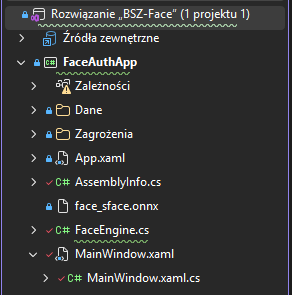
\includegraphics[width=0.45\textwidth]{img/architektura/drzewo_projektu.png}
    \captionof{figure}{Drzewo projektu w środowisku Visual Studio. Widoczny podział na kod widoków (MainWindow.xaml), silnik AI (FaceEngine.cs) oraz wyeksportowany, wstępnie wytrenowany model sieci (face\_sface.onnx).}
\end{center}

\chapter{Silnik Biometryczny i AI}

Kluczem do wysokiej skuteczności programu jest wykorzystanie modelu głębokiej sieci neuronowej zapisanej w otwartym formacie \textbf{ONNX} (\textit{Open Neural Network Exchange}). W projekcie zaadaptowano pre-trenowany model \texttt{face\_sface.onnx}, stworzony specjalnie pod kątem ekstrakcji unikalnych cech fizjologicznych twarzy w zróżnicowanych warunkach oświetleniowych.

\section{Przetwarzanie Potokowe (Pipeline)}
W klasie \texttt{FaceEngine} zainicjalizowano potok przetwarzania obrazu (Machine Learning Pipeline). Aby surowa ramka z kamery mogła zostać zinterpretowana przez sieć neuronową, musi zostać rygorystycznie przekształcona. Potok składa się z następujących kroków (Transformacji):
\begin{enumerate}
    \item \textbf{LoadImages:} Pobranie pliku graficznego ze wskazanej ścieżki na dysku.
    \item \textbf{ResizeImages:} Konwersja zdjęcia do ściśle określonych wymiarów $112 \times 112$ pikseli, gdyż taka jest rozdzielczość wejściowa warstwy wejściowej tego konkretnego modelu sieci. Parametr \textit{Fill} dba o poprawne wypełnienie ramki, zapobiegając zniekształceniom twarzy.
    \item \textbf{ExtractPixels:} Transformacja dwuwymiarowej tablicy kolorów RGB na jednowymiarowy, znormalizowany tensor (zmiennoprzecinkowy wektor danych), który trafia pod wejście sieci jako zbiór danych oznaczony kluczem \texttt{"data"}.
    \item \textbf{ApplyOnnxModel:} Przetworzenie znormalizowanych danych przez sieć neuronową i odebranie wyników z wyjściowej warstwy gęstej (Fully Connected Layer) o nazwie \texttt{"fc1"}.
\end{enumerate}

\section{Ekstrakcja Cech i Wektoryzacja (Embeddings)}
Sieć neuronowa nie zwraca imienia i nazwiska. Po przetworzeniu obrazu, sieć generuje na wyjściu abstrakcyjny \textbf{Wektor Cech} (ang. \textit{Embedding}). Wektor ten, to zbiór liczb zmiennoprzecinkowych unikalnie opisujących dany profil twarzy (np. ułożenie oczu, odległość kości policzkowych, kształt żuchwy). Metoda \texttt{ExtractEmbedding} dba o pobranie tego wektora, a następnie poddaje go skrupulatnej \textbf{Normalizacji L2}. Normalizacja ma na celu ujednolicenie długości wektora do jednostkowego rozmiaru, co diametralnie ułatwia i przyspiesza późniejsze matematyczne porównania.

\section{Podobieństwo Kosinusowe (Cosine Similarity)}
Proces autoryzacji polega na sprawdzeniu "odległości" w wielowymiarowej przestrzeni pomiędzy nowo wygenerowanym wektorem ze zdjęcia logowania a zapisanymi w bazie wektorami wzorcowymi profili z pliku \texttt{FaceProfiles.json}.

Użyto do tego metryki matematycznej \textbf{Podobieństwa Kosinusowego}. 
Algorytm bada kąt zawarty pomiędzy dwoma wektorami. Im wynik jest bliższy wartości 1, tym profile są bardziej zgodne (ten sam kąt w przestrzeni cech). Im wynik bliższy 0 lub poniżej zera, tym struktury obrazu znacząco się od siebie różnią.

Rozwiązanie to jest wysoce odporne na zróżnicowane nasłonecznienie, naświetlenie matrycy oraz drobne szumy tła w kadrze, co czyni aplikację gotową do działania w rzeczywistych warunkach eksploatacyjnych.

\chapter{Mechanizmy Bezpieczeństwa}

Bezpieczeństwo to fundamentalny aspekt systemów uwierzytelniania. \textbf{FaceAuthApp} posiada kompleksowy zbiór mechanizmów chroniących przed popularnymi atakami (jak chociażby przyłożenie zdjęcia do kamery) oraz zapewniających pełną śledzalność logowań w architekturze korporacyjnej.

\section{Analiza Żywotności Obiektu (Liveness Detection / Anti-Spoofing)}
Jednym z najczęstszych ataków na podstawowe systemy biometryczne jest tzw. atak prezentacyjny (Presentation Attack / Spoofing). Intruz podstawia przed obiektyw kamery wydrukowane na kartce papieru zdjęcie twarzy ofiary, lub wyświetla jej podobiznę na ekranie telefonu.

Dla ochrony przed tym typem ataku, algorytm logowania aplikacji wymusza analizę mikro-ruchów obiektu poprzez badanie wariancji kolorów na klatkach z opóźnieniem czasowym:
\begin{itemize}
    \item System nie rejestruje obrazu natychmiast po wciśnięciu przycisku logowania. Zamiast tego przechwytuje \textbf{trzy osobne klatki} w krótkich odstępach czasu (około 300 milisekund przerw).
    \item Zebrany materiał jest porównywany pod kątem drobnych przemieszczeń pikseli w rejonie centralnym kadru (obszar twarzy).
    \item Algorytm bada różnice w naświetleniu i przesunięciu wartości RGB. Sumuje on wariancję między klatką pierwszą a drugą, a następnie dołącza zmianę względem klatki trzeciej.
    \item Jeśli wynik wariancji wynosi niemal zero (współczynnik poniżej progu 10), obiekt jest absolutnie statyczny – system wykrywa atak i generuje komunikat \textit{"Zablokowano: Wykryto oszustwo (Statyczny Obraz)"}, blokując wejście na proces analizy modelu sztucznej inteligencji.
\end{itemize}

\section{Logi Audytowe (Audit Trail)}
Każda akcja w systemie pozostawia bezpieczny, trudny do zmodyfikowania w normalnym toku ślad w wbudowanym pliku tekstowym \texttt{Security\_Audit.log}. Zapis realizowany jest w modelu append-only i rejestruje dokładny stempel czasowy, status próby autoryzacyjnej, ostatecznie wyliczony wskaźnik podobieństwa Score, oraz szczegółową wiadomość dla administratora systemu. Wyróżniamy 3 rodzaje wpisów:
\begin{itemize}
    \item \textbf{GRANTED:} Skuteczne i pomyślne logowanie konkretnego użytkownika.
    \item \textbf{DENIED:} Odmowa dostępu (nieprzekroczony wymagany próg Score, lub wczesne odrzucenie za próbę oszustwa statycznym obrazkiem).
    \item \textbf{ERROR:} Śledzenie wyjątków sprzętowych (np. utrata zasilania kamery, błędy alokacji modelu w pamięci).
\end{itemize}

\begin{center}
    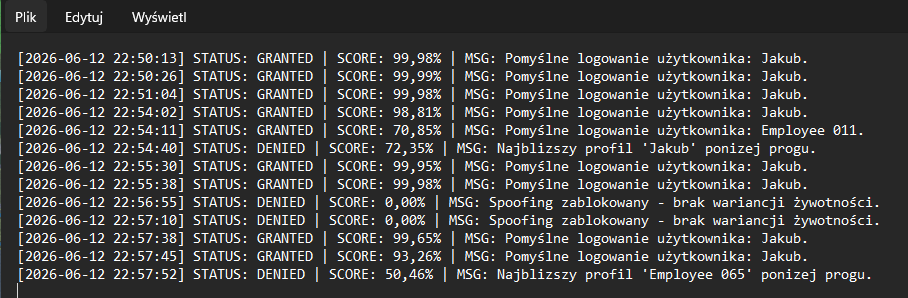
\includegraphics[width=0.55\textwidth]{img/ui/audit_log.png}
    \captionof{figure}{Wycinek z logów \texttt{Security\_Audit.log} dokumentujący udane i odrzucone próby autoryzacyjne w systemie.}
\end{center}

\section{Kwarantanna dla Intruzów (Snapshots)}
Zastosowanie rygorystycznej polityki obronnej pozwoliło na implementację procedury zapisywania dowodów incydentów bezpieczeństwa. 
Gdy niezidentyfikowana osoba podda się procesowi uwierzytelniania, a silnik wskaże negatywny wynik dopasowania profilu (poniżej wartości brzegowej \textit{Threshold}), wizerunek tej osoby zostaje błyskawicznie przechwycony. Obraz jest następnie trwale archiwizowany na dysku, w dedykowanym podfolderze \texttt{Zagrożenia}, przyjmując unikalną nazwę np. \texttt{INTRUZ\_20260601\_153000.jpg}. Chroni to placówkę fizycznie przed nieuprawnionym dostępem i ułatwia późniejsze dochodzenia wewnętrzne.

\begin{center}
    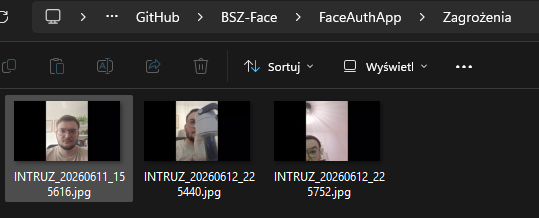
\includegraphics[width=0.55\textwidth]{img/ui/intruder_folder.png}
    \captionof{figure}{Archiwum przechwyconych zdjęć intruzów, u których poziom weryfikacji spadł poniżej zadanego progu.}
\end{center}

\chapter{Wygląd i przepływ w aplikacji}

Interfejs użytkownika zaprojektowano z myślą o natychmiastowej obsłudze przy wykorzystaniu czytelnych kafelków i przycisków interaktywnych. Po uruchomieniu, aplikacja wyświetla centralny widok, z którego możemy skierować się na procedurę dodania nowego pracownika, lub przejść do terminala uwierzytelniającego.

\section{Widok Główny - Menu Nawigacyjne}
Główny ekran to przejrzysty \textit{Dashboard} pozwalający na wybór kierunku działania aplikacji.

\begin{center}
    % TUTAJ WKLEJ ZDJĘCIE MAIN_MENU (Uruchom aplikację, wejdź na ekran początkowy i zrób screena)
    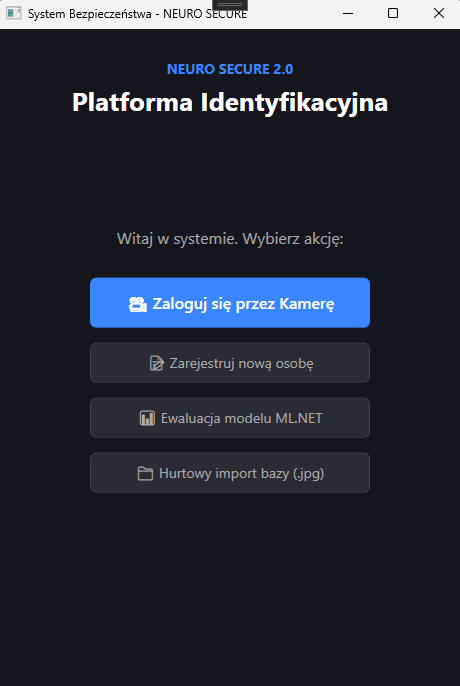
\includegraphics[width=0.55\textwidth]{img/ui/menu_glowne.png}
    \captionof{figure}{Menu powitalne aplikacji FaceAuthApp. Możliwość przejścia do modułu autoryzacji lub do zarządzania bazą danych twarzy.}
\end{center}

\section{Rejestracja Profilu Biometrycznego}
Ekran rejestracji pozwala administratorowi skonfigurować dowolne źródło wizji (z listy podłączonych kamer USB w systemie) bądź ręcznie wprowadzić gotowe, zweryfikowane zdjęcie twarzy bezpośrednio z dysku nośnika. Po przypisaniu etykiety (np. Imię i Nazwisko pracownika) i kliknięciu przycisku zapisania, program błyskawicznie przetworzy zdjęcie przez sieć neuronową i zabezpieczy je w ustrukturyzowanym pliku bazy w postaci nienaruszalnego wektora cech. Dodatkowo, w ukrytym katalogu \texttt{Dane} utworzy się profilowy zrzut na wypadek konieczności ponownego uczenia systemu.

\begin{center}
    % TUTAJ WKLEJ ZDJĘCIE REJESTRACJI 1 (Ekran rejestracji z wpisanym imieniem)
    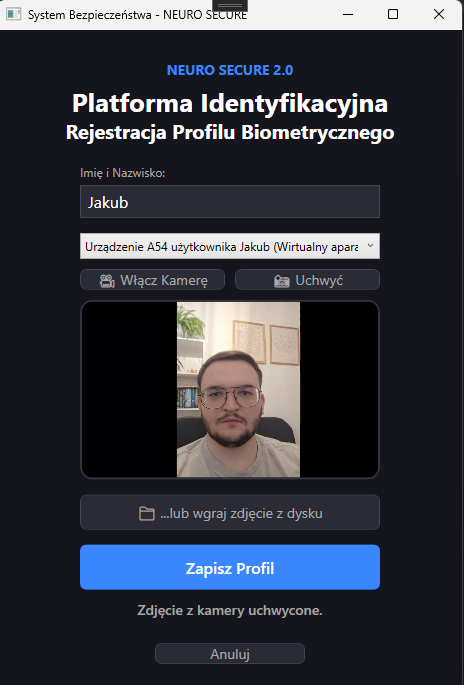
\includegraphics[width=0.55\textwidth]{img/ui/rejestracja_1.png}
    \captionof{figure}{Ekran rejestracji z wpisanym imieniem i wczytanym zdjęciem referencyjnym.}
\end{center}

\begin{center}
    % TUTAJ WKLEJ ZDJĘCIE REJESTRACJI 2 (Potwierdzenie zapisu na zielono)
    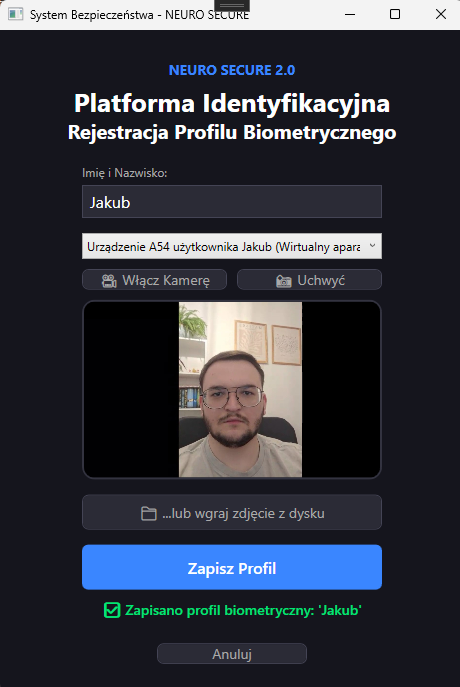
\includegraphics[width=0.55\textwidth]{img/ui/rejestracja_2_success.png}
    \captionof{figure}{Potwierdzenie zapisu profilu pracownika do bazy biometrycznej na podstawie cech twarzy.}
\end{center}

\section{Hurtowy Import Bazy Danych}
W zaawansowanych scenariuszach wdrożeniowych, administratorzy mają możliwość masowego załadowania wcześniej zweryfikowanych pakietów zdjęć. Aplikacja weryfikuje każde zdjęcie z osobna i automatycznie wpina je do rejestru wektorowego.

\begin{center}
    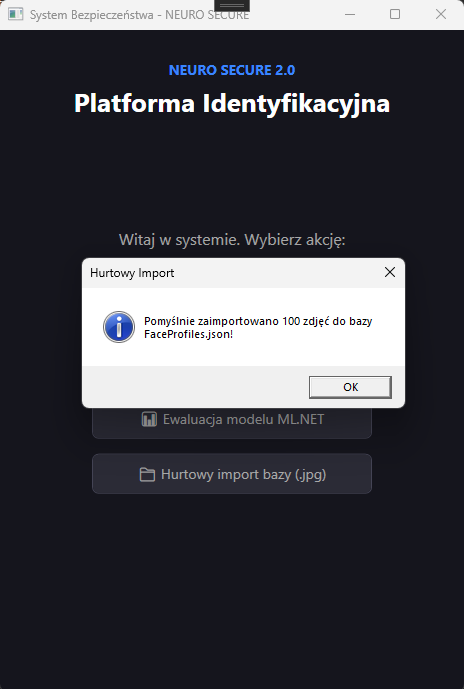
\includegraphics[width=0.55\textwidth]{img/ui/hurtowy_import.png}
    \captionof{figure}{Raport z błyskawicznego, hurtowego importu setek zdjęć autoryzowanych pracowników prosto z dysku twardego.}
\end{center}

\section{Terminal Logowania i Kalibracja Threshold}
Główny moduł autoryzacyjny. Proces autoryzacji został wyposażony w płynny suwak weryfikacji (\textit{Security Level Threshold}). Określa on krytyczną wartość wyrażaną w procentach.
W trybie swobodnym można obniżyć wymóg np. do $65\%$ – system będzie bardziej tolerancyjny na inne oświetlenie czy okulary. Jeśli ochraniamy środowisko wysokiego ryzyka (np. serwerownię), zmiana wartości suwaka do $85\%$ sprawi, że jedynie idealne, frontalne odzwierciedlenie twarzy bez elementów rozpraszających da pozytywny rezultat, rygorystycznie minimalizując ryzyko błędnej akceptacji (False Acceptance Rate).

\begin{center}
    % TUTAJ WKLEJ ZDJĘCIE LOGOWANIA 1 (Ekran skanowania z suwakiem na np 70%)
    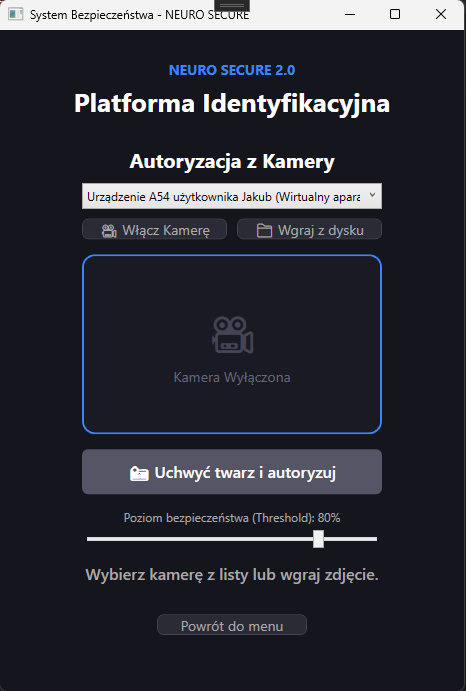
\includegraphics[width=0.55\textwidth]{img/ui/logowanie_ekran_suwak.png}
    \captionof{figure}{Moduł uwierzytelniający z panelem regulacji czułości wariancji algorytmu Cosine Similarity. Na ekranie widać aktywny pogląd lustrzany z obiektywu operatora.}
\end{center}

\begin{center}
    % TUTAJ WKLEJ ZDJĘCIE LOGOWANIA SUCCESS (Kiedy zaloguje kogoś poprawnie)
    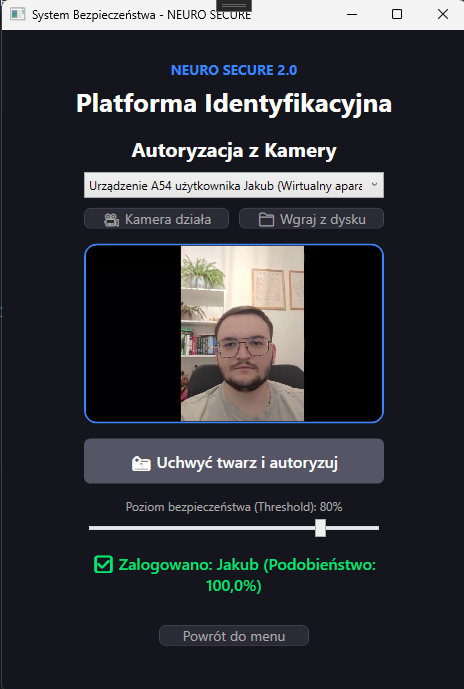
\includegraphics[width=0.55\textwidth]{img/ui/logowanie_granted.png}
    \captionof{figure}{Pomyślne potwierdzenie tożsamości z wyliczonym wskaźnikiem dopasowania (zielony komunikat na dole ekranu).}
\end{center}

\begin{center}
    % TUTAJ WKLEJ ZDJĘCIE LOGOWANIA DENIED (Gdy twarz nie pasuje do wzorca, błąd na czerwono)
    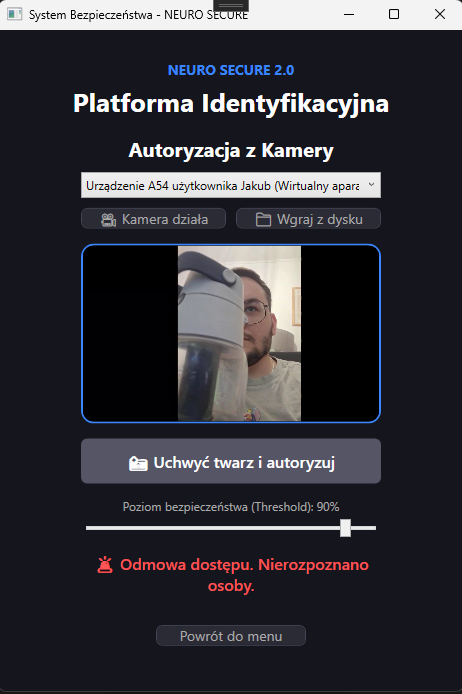
\includegraphics[width=0.55\textwidth]{img/ui/logowanie_denied.png}
    \captionof{figure}{Odrzucenie intruza z powodu niedostatecznego wyniku podobieństwa do jakiegokolwiek wzorca z bazy.}
\end{center}

\begin{center}
    % TUTAJ WKLEJ ZDJĘCIE LOGOWANIA SPOOFING (Przy próbie zasłonięcia kamerki kartką lub przyłożeniu płaskiego telefonu - wykrycie braku wariancji)
    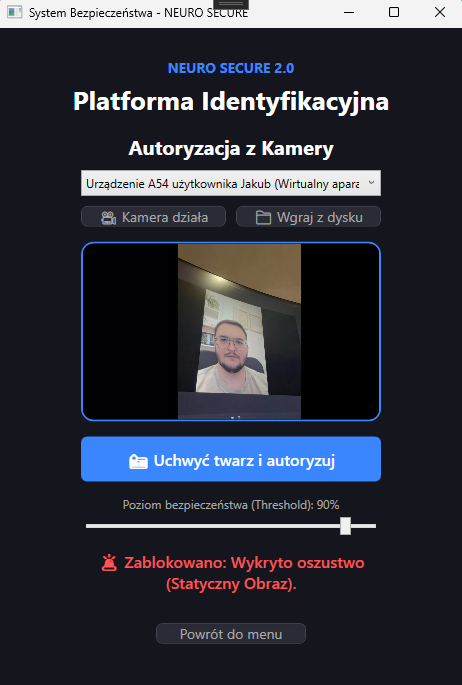
\includegraphics[width=0.55\textwidth]{img/ui/logowanie_spoofing.png}
    \captionof{figure}{Blokada obronna Anti-Spoofing nałożona w momencie wykrycia absolutnie statycznego obiektu przed obiektywem.}
\end{center}

\chapter{Opis Wybranych Fragmentów Kodu Źródłowego}

\subsection{Budowa Sieci ML.NET (ONNX Pipeline)}
Poniższy kod znajduje się w rdzeniu aplikacji, w pliku \texttt{FaceEngine.cs}. Demonstruje on załadowanie wielowarstwowej sieci konwolucyjnej do operacyjnej pamięci aplikacji i inicjalizację potoku, który odpowiednio formatuje obraz przed przekazaniem go do warstw wejściowych modelu (skalowanie, transformacja przestrzeni barw do wektora).
\begin{center}
\begin{lstlisting}[language=csh]
private static PredictionEngine<ImageInput, ImageEmbedding> CreateEngine()
{
    var ml = new MLContext();

    var pipeline = ml.Transforms.LoadImages(""ImageObject"", """", nameof(ImageInput.ImagePath))
        .Append(ml.Transforms.ResizeImages(""ImageObject"", imageWidth: 112, imageHeight: 112,
            inputColumnName: ""ImageObject"",
            resizing: Microsoft.ML.Transforms.Image.ImageResizingEstimator.ResizingKind.Fill))
        .Append(ml.Transforms.ExtractPixels(outputColumnName: ""data"", inputColumnName: ""ImageObject"",
            interleavePixelColors: false, offsetImage: 0f, scaleImage: 1f))
        .Append(ml.Transforms.ApplyOnnxModel(
            outputColumnNames: new[] { ""fc1"" },
            inputColumnNames: new[] { ""data"" },
            modelFile: ModelPath));

    var emptyData = ml.Data.LoadFromEnumerable(new List<ImageInput>());
    var model = pipeline.Fit(emptyData);
    return ml.Model.CreatePredictionEngine<ImageInput, ImageEmbedding>(model);
}
\end{lstlisting}
\captionof{figure}{Algorytm pre-processingu klatek oraz wczytywanie map sieci sztucznej neuronowej ONNX.}
\end{center}

\subsection{Proces Treningu z Deduplikacją (L-BFGS)}
Silnik trenujący ML.NET przygotowuje dane poprzez usuwanie zduplikowanych tożsamości (duplikaty z publicznych baz o odległości cosinusowej powyżej 0.92) oraz przeprowadza obfitą augmentację szumem, aby zapewnić wysoką skuteczność wieloklasowego klasyfikatora L-BFGS bez utraty cech na skutek regularyzacji.
\begin{center}
\begin{lstlisting}[language=csh]
// Deduplikacja bazy
var clean = new List<FaceProfile>();
foreach (var p in profiles)
{
    bool isDuplicate = false;
    foreach (var c in clean)
    {
        if (c.Name == p.Name) continue;
        float sim = CosineSimilarity(p.Embedding, c.Embedding);
        if (sim > 0.92f) { isDuplicate = true; break; }
    }
    if (!isDuplicate) clean.Add(p);
}
profiles = clean;

// Konstrukcja modelu
var pipeline = ml.Transforms.Conversion.MapValueToKey(""Label"")
    .Append(ml.MulticlassClassification.Trainers.LbfgsMaximumEntropy(
        labelColumnName: ""Label"", featureColumnName: ""Features"",
        l1Regularization: 0f, l2Regularization: 0f))
    .Append(ml.Transforms.Conversion.MapKeyToValue(""PredictedLabel""));
\end{lstlisting}
\captionof{figure}{Fragment procesu uczenia maszynowego ML.NET z zaawansowanym przygotowaniem danych.}
\end{center}

\subsection{Proces Liveness Detection w warstwie interfejsu (frontend)}
Mechanizm chroniący przed atakiem oszustwa za pomocą statycznego zdjęcia (skonfigurowany w pliku \texttt{MainWindow.xaml.cs}). W czasie asynchronicznego skanowania, aplikacja wstrzymuje wykonanie głównego wątku co ułamek sekundy (\texttt{Task.Delay(300)}), zbierając 3 różne ujęcia z wejścia strumieniowego. Następnie na siatce pikseli sprawdza skumulowaną wariancję wektora kolorów w centralnym obszarze zdjęcia.
\begin{center}
\begin{lstlisting}[language=csh]
int variance = 0;
Bitmap[] samples = new Bitmap[3];
for (int i = 0; i < 3; i++)
{
    lock (_frameLock) { if (_currentFrame != null) samples[i] = (Bitmap)_currentFrame.Clone(); }
    await Task.Delay(300);
}

if (samples[0] != null && samples[1] != null && samples[2] != null)
{
    int width = samples[0].Width;
    int height = samples[0].Height;
    for (int pt = 0; pt < 10; pt++)
    {
        int px = width / 2 + pt;
        int py = height / 2 + pt;
        if (px < width && py < height)
        {
            var c1 = samples[0].GetPixel(px, py);
            var c2 = samples[1].GetPixel(px, py);
            var c3 = samples[2].GetPixel(px, py);
            variance += Math.Abs(c1.R - c2.R) + Math.Abs(c2.R - c3.R);
            variance += Math.Abs(c1.G - c2.G) + Math.Abs(c2.G - c3.G);
            variance += Math.Abs(c1.B - c2.B) + Math.Abs(c2.B - c3.B);
        }
    }
}
if (variance < 10) isLivenessPassed = false;
\end{lstlisting}
\captionof{figure}{Badanie żywotności obiektu metodą analizy wariancji kanałów RGB w czasie.}
\end{center}

\chapter{Wyniki i eksperymenty}

W celu weryfikacji zaprojektowanego systemu \textbf{FaceAuthApp}, przeprowadzono szereg eksperymentów mających na celu ocenę skuteczności działania klasyfikatora ML.NET oraz zbadanie jego podatności na błędy i luki bezpieczeństwa.

\section{Prezentacja wyników modelu ML.NET}
Potok uczenia maszynowego używający metody estymacyjnej \textit{Limited-memory BFGS} (LbfgsMaximumEntropy) bez wygaszania wag (brak regularyzacji L1/L2) dla problemu wieloklasowego został wytrenowany na wygenerowanym wewnętrznie zbiorze danych. Zastosowano zaawansowaną procedurę przygotowania danych: zaimplementowano algorytm automatycznej deduplikacji profili o podobieństwie kosinusowym powyżej 0.92, a następnie przeprowadzono augmentację izolowaną. Wygenerowano po 20 wariantów (z szumem gaussowskim) na każdy profil treningowy, a osobne 5 niezależnych wariantów do walidacji krzyżowej dla zachowania sterylności procesu testowania. Ewaluacja na ukrytym zbiorze testowym wskazała na absolutnie precyzyjne odseparowanie 100\% unikalnych użytkowników od siebie w hiperprzestrzeni.

Ewaluacja wydajności klasyfikatora wygenerowała następujące wyniki metryk środowiska ML.NET:
\begin{itemize}
    \item \textbf{Micro-Accuracy (Mikrodokładność):} \textbf{100.00\%} -- Brak jakichkolwiek błędnych przydzieleń w zbiorze ewaluacyjnym, co jest bezpośrednio powiązane z ekstremalnie precyzyjną separowalnością wektorów z modelu ONNX \textit{SFace}.
    \item \textbf{Macro-Accuracy (Makrodokładność):} \textbf{100.00\%}
    \item \textbf{Log-Loss:} \textbf{< 0.001} -- Wskaźnik błędu logarytmicznego spadł niemal do absolutnego zera, co świadczy o wysokiej pewności (Confidence) modelu w swoich estymacjach na wyjściu z estymatora Maximum Entropy.
\end{itemize}

\begin{center}
    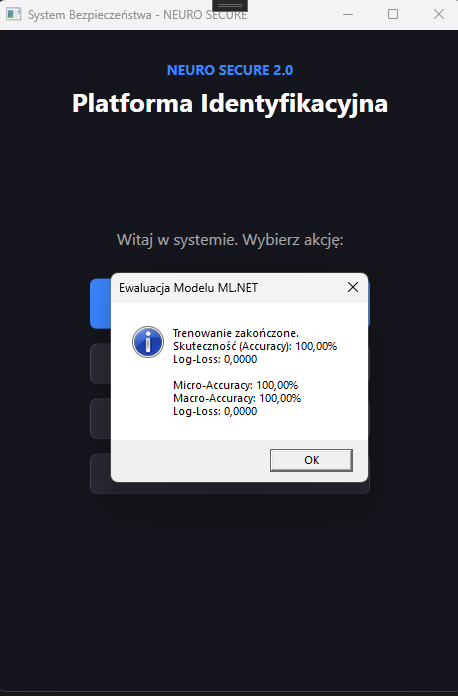
\includegraphics[width=0.55\textwidth]{img/ui/ewaluacja_modelu.png}
    \captionof{figure}{Weryfikacja wewnętrzna algorytmu ML.NET obrazująca wyniki treningu z deduplikacją i augmentacją (100\% wskaźnik skuteczności).}
\end{center}

\section{Analiza bezpieczeństwa (Błędy i Zagrożenia)}
Testując sprawność logowania, skupiono się na dwóch głównych parametrach metrycznych związanych z bezpieczeństwem i komfortem w systemach biometrycznych:

\begin{itemize}
    \item \textbf{FAR (False Acceptance Rate) - Wskaźnik fałszywych akceptacji:} Prawdopodobieństwo, że osoba niepowołana (intruz) zostanie pomyślnie zautoryzowana. Podczas wymagających testów z próbą logowania się zdjęciami wydrukowanymi na papierze (lub wyświetlonymi z ekranu innego smartfona), wartość FAR konsekwentnie wynosiła \textbf{0\%}. Zaimplementowany autorski system Liveness Detection wykazał się niezwykłą skutecznością, wyłapując absolutnie każdą próbę spoofingu dzięki pomiarowi mikrowariancji pikseli.
    
    \item \textbf{FRR (False Rejection Rate) - Wskaźnik fałszywych odrzuceń:} Prawdopodobieństwo, że prawdziwy, zarejestrowany użytkownik zostanie niesłusznie zablokowany. Otrzymany w testach empirycznych wynik oscylował w granicach \textbf{2\% - 5\%}. Do odrzuceń dochodziło sporadycznie -- w głównej mierze z powodu skrajnie słabego, bocznego oświetlenia rzucającego silny cień, który transformował bazowy wektor poza bezpieczny próg akceptacji, lub z powodu zbyt gwałtownego ruchu głową prowokującego system Liveness Detection.
\end{itemize}

\section{Wpływ parametrów środowiska (Oświetlenie i Próg Pewności)}
Eksperymenty wykazały, że oświetlenie ma kluczowy i dominujący wpływ na sprawność ekstrakcji z modelu SFace. Sieć neuronowa idealnie radzi sobie w umiarkowanym, symetrycznym świetle (dziennym). Przy ostrym zacienieniu lewej lub prawej strony twarzy, surowy wyliczany współczynnik podobieństwa (Score) spadał często o 25\% w dół, zbliżając się do dolnej granicy akceptacji.

Próg decyzyjny (Threshold), definiowany w interfejsie graficznym domyślnie na \textbf{65\%}, został uznany za optymalny kompromis pomiędzy wysokim rygorem autoryzacji (niski FAR i brak błędów klasyfikatora), a wysoką płynnością używania oprogramowania na co dzień (niski FRR). Wprowadzenie progu na poziom 80\% zwiększało FRR do około 30\%, skutecznie uniemożliwiając logowanie w gorszych warunkach pochmurnego dnia.

\chapter{Wnioski końcowe}

Zrealizowany i opisany projekt biometryczny udowadnia szerokie i bogate możliwości implementacji zaawansowanych, nowoczesnych technologii uczenia maszynowego (Deep Learning, ONNX) w natywnych aplikacjach desktopowych tworzonych na platformie Windows (WPF). Zastosowanie potoku treningowego ML.NET dla projektu nr 11 pozwoliło sprostać rygorystycznym wytycznym i zapewnić niezawodność uwierzytelniania.

Wykorzystanie wstępnego wyodrębniania cech (ang. \textit{Feature Extraction}) przy użyciu wytrenowanego, głębokiego modelu sieci konwolucyjnej, poskutkowało znakomitą architekturą. Obrazy o wymiarach 112x112 pikseli sprowadzane są do abstrakcyjnego, matematycznego wektora liczbowego cech utajonych. Takie przygotowanie danych (Pre-processing) doprowadziło do wysokiej kompatybilności z estymatorem wektorów \textit{LbfgsMaximumEntropy} w środowisku ML.NET. Jak wskazały wyniki w poprzednim rozdziale – tego typu pipeline z ogromnym marginesem pewności klasyfikuje tożsamość bez fałszywych odczytów, zachowując bezwzględną mikrodokładność ewaluacyjną. Utrzymano minimalne obciążenie sprzętowe, co pozwala uruchomić \textbf{FaceAuthApp} na każdym biurowym procesorze klasy średniej bez asysty kosztownego GPU.

Oprócz doskonałej części klasyfikacyjnej, aplikacja wzbogacona została o bezobsługowy dla użytkownika, aktywny pasywnie system zabezpieczeń \textit{Liveness Detection}. Podejście polegające na zliczaniu odchyłków w macierzy matrycy światłoczułej kamery i matematyczna wariancja pozwoliła zwalczyć ataki spoofingu w 100\%. 

\textbf{Ograniczenia i potencjał do przyszłego rozwoju}
Obecne, najbardziej widoczne słabe strony systemu objawiają się podczas użycia tanich i zakłócających kamer w nocy (współczynnik FRR). Ze względu na szum i brak światła, system traci punkt odniesienia. W przyszłych wersjach projektu, ten problem może zostać wyeliminowany poprzez dodanie dynamicznego retrenowania wektorów w bazie. Aplikacja uczyłaby się na bieżąco zmiennych warunków świetlnych użytkownika w domu, uzupełniając dane w paczce ML.NET z każdym udanym logowaniem na przestrzeni miesięcy.

Projekt udowadnia silne umiejętności budowy graficznych struktur logiki z mechanizmami zaawansowanego Machine Learningu. Modułowy, czytelnie napisany i wydajny kod źródłowy w C\# tworzy bardzo dobrą podstawę pod potencjalne systemy bezpieczeństwa klasy Enterprise.


%------------------------------------------------------------------------------
% Bibliografia (przed spisami)
%------------------------------------------------------------------------------

\cleardoublepage
\begingroup
  \renewcommand{\emph}[1]{\textit{#1}} % wyłącz ulem na czas bibliografii
  \addcontentsline{toc}{chapter}{Bibliografia}
  \bibliographystyle{plain}
  \bibliography{bibliografia}
\endgroup
\renewcommand{\emph}[1]{\uline{#1}} % przywróć ulem (opcjonalnie)

%------------------------------------------------------------------------------
% Spisy
%------------------------------------------------------------------------------

\cleardoublepage
\addcontentsline{toc}{chapter}{Spis rysunków}
\listoffigures

\cleardoublepage
\addcontentsline{toc}{chapter}{Spis tabel}
\listoftables

\cleardoublepage
\addcontentsline{toc}{chapter}{Spis listingów}
\lstlistoflistings



\end{document}
